\section{正规方程法}
\label{sec:ls-normal-equations-method}

前五节处理的都是方阵的精确解。现在转向超定的最小二乘问题，矩阵不再是方阵，消元也不再直接适用。最直接的办法是先把问题化为一个方阵问题：最小二乘解满足正规方程，而满列秩时正规方程的系数矩阵对称正定，正好可以交给Cholesky分解。

\subsection{主要思想}

输入满列秩的$\bm A\in\mathbb R^{m\times d}$（$m\geq d$）和$\bm b\in\mathbb R^m$，求唯一的最小二乘解$\hat{\bm x}$。

\paragraph{从残差正交到正规方程}
记残差$\bm r=\bm b-\bm A\bm x$。第~\ref{sec:ls-ordinary-ls}节已经证明，最优拟合值是$\bm b$在列空间上的正交投影，所以最优时残差与$\bm A$的每一列$\bm a_j$正交：$\bm a_j^\top(\bm b-\bm A\hat{\bm x})=0$，$j=1,\ldots,d$。把这$d$个标量等式堆叠起来，就是正规方程
\[
 \bm A^\top\bm A\hat{\bm x}=\bm A^\top\bm b
\]
（式~\eqref{eq:linear-algebra-normal-equations}）。这一推导只用正交投影，不需要多元求导。

\paragraph{满列秩保证正定}
记$\bm G=\bm A^\top\bm A$。若$\bm A$满列秩，则对任意$\bm z\neq\bm0$有$\bm A\bm z\neq\bm0$，于是$\bm z^\top\bm G\bm z=\lVert\bm A\bm z\rVert_2^2>0$，$\bm G$对称正定。这样$m\times d$的最小二乘问题就变成一个$d$阶正定方程，可以用第~\ref{sec:ls-cholesky}节的Cholesky分解$\bm G=\bm L\bm L^\top$求出唯一解。秩亏时这一正定论证失效，应改用后面的QR或SVD分支。

\paragraph{按行累计}
把$\bm A$的第$i$行记为$\bm A_{i,:}$，逐元素展开矩阵乘法可知
\[
 \bm G=\sum_{i=1}^m\bm A_{i,:}^\top\bm A_{i,:},\qquad
 \bm A^\top\bm b=\sum_{i=1}^mb_i\bm A_{i,:}^\top .
\]
每条观测只贡献一个$d$阶外积和一个$d$维向量，所以可以每读入一行就把它的贡献累加进去，不必同时保存全部观测行。这是正规方程法在数据量很大时的主要优点。代数上等价并不意味着数值条件相同：$\bm G$的条件数是$\bm A$的平方（定理~\ref{thm:ls-normal-equations-condition-squaring}），这是后面引入QR求解的原因。

\subsection{算法实现}

\paragraph{形成Gram矩阵}
第一步形成Gram矩阵$\bm G=\bm A^\top\bm A$与右端$\bm c=\bm A^\top\bm b$：先令$\bm G=\bm0$、$\bm c=\bm0$，再对$i=1,\ldots,m$依次累加
\[
 \bm G\leftarrow\bm G+\bm A_{i,:}^\top\bm A_{i,:},\qquad
 \bm c\leftarrow\bm c+b_i\bm A_{i,:}^\top .
\]
$\bm G$对称，只需累加下三角部分。

\paragraph{\texorpdfstring{$\bm L\bm L^\top$}{LL\textasciicircum T}分解}
然后用第~\ref{sec:ls-cholesky}节的逐列过程计算$\bm G=\bm L\bm L^\top$。满列秩保证了这一步的正定前提；若分解中出现非正的开方量，说明$\bm A$秩亏或条件很差，应转入QR或SVD求解。

\paragraph{前代与回代}
有了因子，先用第~\ref{sec:ls-lu}节的前代求解$\bm L\bm y=\bm c$，再用回代求解$\bm L^\top\hat{\bm x}=\bm y$，得到最小二乘解$\hat{\bm x}$。两次三角求解的次序来自$\bm L(\bm L^\top\hat{\bm x})=\bm c$，与用Cholesky分解解正定方程的步骤相同。

\begin{example}[直线拟合的正规方程法]
\label{ex:ls-normal-equations-line-fit}
沿用示例~\ref{ex:ls-line-least-squares}的直线拟合，$\bm A=\left[\begin{smallmatrix}1&0\\1&1\\1&2\end{smallmatrix}\right]$，$\bm b=(1,2,2)^\top$，按正规方程法的次序计算：先逐行累计$\bm G$与$\bm c$，再分解$\bm G$并作两次三角求解。三行依次给出$\bm G$的增量
\[
 \begin{bmatrix}1&0\\0&0\end{bmatrix},\quad
 \begin{bmatrix}1&1\\1&1\end{bmatrix},\quad
 \begin{bmatrix}1&2\\2&4\end{bmatrix},
\]
以及$\bm c$的增量$(1,0)^\top$、$(2,2)^\top$、$(2,4)^\top$，因此$\bm G=\left[\begin{smallmatrix}3&3\\3&5\end{smallmatrix}\right]$，$\bm c=(5,6)^\top$。

对$\bm G$作Cholesky分解，得$l_{1,1}=\sqrt3$、$l_{2,1}=3/\sqrt3=\sqrt3$、$l_{2,2}=\sqrt{5-3}=\sqrt2$，即$\bm L=\left[\begin{smallmatrix}\sqrt3&0\\\sqrt3&\sqrt2\end{smallmatrix}\right]$。前代得$y_1=5/\sqrt3$，$y_2=(6-\sqrt3\cdot5/\sqrt3)/\sqrt2=1/\sqrt2$；回代得$\hat x_2=1/2$，$\hat x_1=(5/\sqrt3-\sqrt3/2)/\sqrt3=5/3-1/2=7/6$。

最后用原始数据重算残差：$\bm r=\bm b-\bm A\hat{\bm x}=(-\tfrac16,\tfrac13,-\tfrac16)^\top$，它与两列都正交，$\bm A^\top\bm r=\bm0$，且$\lVert\bm r\rVert_2^2=\tfrac16$。原残差不为零，是因为三个点本来就不共线，方程不相容；最小二乘完成的标志是$\bm A^\top\bm r=\bm0$，而不是$\bm r=\bm0$。若累计后的Cholesky分解失败，或结果对舍入很敏感，也不能只凭正规方程这个小系统的残差小就宣布结果可靠。
\end{example}

\subsection{算法分析}

\paragraph{正确性}
两次三角求解给出$\bm L\bm L^\top\hat{\bm x}=\bm c$，即$\bm A^\top\bm A\hat{\bm x}=\bm A^\top\bm b$，所以$\hat{\bm x}$满足正规方程，由定理~\ref{thm:ls-least-squares-solutions}是唯一的最小二乘解。

\paragraph{数值敏感度}
这条路线的代价在精度。对满列秩矩阵定义$\kappa_2(\bm A)=\sigma_{\max}(\bm A)/\sigma_{\min}(\bm A)$，方阵时它与第~\ref{sec:ls-matrix-condition-number}节的定义一致。

\begin{theorem}[正规方程使条件数平方]
\label{thm:ls-normal-equations-condition-squaring}
设$\bm A\in\mathbb R^{m\times d}$满列秩，则$\kappa_2(\bm A^\top\bm A)=\kappa_2(\bm A)^2$。
\end{theorem}
\begin{proof}
由第~\ref{chap:singular-value-decomposition}章的奇异值分解$\bm A=\bm U\bm\Sigma\bm V^\top$，得
\[
 \bm A^\top\bm A=\bm V\operatorname{diag}(\sigma_1^2,\ldots,\sigma_d^2)\bm V^\top .
\]
满列秩时$\sigma_d>0$，这是对称正定矩阵的谱分解，其最大、最小特征值即最大、最小奇异值，分别为$\sigma_1^2$与$\sigma_d^2$，故$\kappa_2(\bm A^\top\bm A)=\sigma_1^2/\sigma_d^2=\kappa_2(\bm A)^2$。
\end{proof}

$\bm A$压缩得很厉害的方向在$\bm G$中被压缩两次，形成$\bm G$时累计内积的舍入就可能抹掉这些方向上的信息。因此正规方程法适合条件较好的满列秩问题；误差界怎样带上$\kappa_2(\bm A)^2$，见第~\ref{sec:ls-ls-regularization-sensitivity}节。

\paragraph{计算代价与适用范围}
形成Gram矩阵可能增加填充：$\bm A$只要有一行全是非零元，这一行的外积就使$\bm G$成为稠密矩阵。稠密情形下形成$\bm G$约需$md^2$次运算，分解约需$d^3/3$次，总工作为$O(md^2+d^3)$。秩亏时正规方程仍刻画全部最小二乘解，但$\bm G$只是半正定的，Cholesky分解会遇到零主元，本算法的前提不再成立；这时的选解由第~\ref{sec:ls-svd-solve}节的SVD路线完成。

\section{QR求解}
\label{sec:ls-qr-method}

正规方程法的精度损失来自形成$\bm A^\top\bm A$。QR求解不形成它，而是直接对$\bm A$作正交三角化。本节先利用QR因子写清最小二乘与满行秩最小范数解的共同求解过程，再分别说明修正Gram--Schmidt正交化、Householder反射与Givens旋转怎样计算这些因子。

\subsection{主要思想}

输入满列秩的$\bm A\in\mathbb R^{m\times d}$（$m\geq d$）和$\bm b\in\mathbb R^m$，求唯一的最小二乘解$\hat{\bm x}$。正交变换保持欧氏长度，用它同时变换$\bm A$和$\bm b$不会改变残差的长度。因此可以找一个正交矩阵把$\bm A$化为上三角形，最小二乘问题就变成一个三角方程，全程不必形成$\bm A^\top\bm A$。

\paragraph{残差的分解}
第~\ref{chap:inner-product-spaces}章的薄QR分解（式~\eqref{eq:ls-qr-factorization}）给出$\bm A=\bm Q_1\bm R$，其中$\bm Q_1\in\mathbb R^{m\times d}$的列标准正交，$\bm R$为$d$阶上三角矩阵；满列秩时$\bm R$可逆。把$\bm Q_1$的列补成$\mathbb R^m$的标准正交基，新增的列排成$\bm Q_2$，得到完整的分解
\[
 \bm A=\bm Q\begin{bmatrix}\bm R\\\bm0\end{bmatrix},\qquad \bm Q=[\bm Q_1\;\bm Q_2].
\]
把右端也变换为$\bm Q^\top\bm b=(\bm c_1^\top,\bm c_2^\top)^\top$，$\bm c_1=\bm Q_1^\top\bm b$含前$d$个分量。由$\bm Q^\top$保持长度，对任意$\bm x$有
\begin{equation}
 \begin{aligned}
 \lVert\bm A\bm x-\bm b\rVert_2^2
 &=\lVert\bm Q^\top(\bm A\bm x-\bm b)\rVert_2^2\\
 &=\lVert\bm R\bm x-\bm c_1\rVert_2^2+\lVert\bm c_2\rVert_2^2 .
 \end{aligned}
 \label{eq:ls-qr-residual-split}
\end{equation}
第二项与$\bm x$无关，是任何$\bm x$都无法拟合的部分；第一项可以通过求解$\bm R\bm x=\bm c_1$消为零。

\paragraph{回代与最小残差}
$\bm R\bm x=\bm c_1$是上三角方程，按式~\eqref{eq:ls-back-substitution}逆序展开，$\hat x_i=\bigl((\bm c_1)_i-\sum_{j>i}r_{i,j}\hat x_j\bigr)/r_{i,i}$。最小残差范数为$\lVert\bm c_2\rVert_2$。使用薄分解时不必补出$\bm Q_2$：不可拟合部分就是$\bm b-\bm Q_1\bm Q_1^\top\bm b$，即$\bm b$减去它在列空间上的正交投影（第~\ref{sec:ls-orthogonal-projection}节）。

\paragraph{满行秩的最小范数解}
同一种分解也能处理欠定方程。设$\bm A\in\mathbb R^{m\times d}$满行秩，$m<d$，求解目标改为第~\ref{sec:ls-select-among-solutions}节的最小范数精确解$\bm x_\star$。这时对$\bm A^\top$而不是$\bm A$作薄QR分解$\bm A^\top=\bm Q\bm R$，其中$\bm Q\in\mathbb R^{d\times m}$的列标准正交，$\bm R$为$m$阶可逆上三角矩阵，于是$\bm A=\bm R^\top\bm Q^\top$。任一$\bm x$可唯一写成$\bm x=\bm Q\bm y+\bm w$，其中$\bm Q^\top\bm w=\bm0$。由$\bm A\bm w=\bm R^\top\bm Q^\top\bm w=\bm0$，方程化为$\bm A\bm x=\bm R^\top\bm y=\bm b$，只约束坐标$\bm y$；而勾股关系给出$\lVert\bm x\rVert_2^2=\lVert\bm y\rVert_2^2+\lVert\bm w\rVert_2^2$。所以先前代求解$\bm R^\top\bm y=\bm b$，再令$\bm w=\bm0$，输出$\bm x_\star=\bm Q\bm y$。对转置作分解，是因为最小范数解位于$\operatorname{range}(\bm A^\top)$中，需要的是这个子空间的标准正交基。

\paragraph{只需应用正交因子}
两个分支都只用到$\bm Q^\top$或$\bm Q$对向量的作用，并不要求显式存出完整的$\bm Q$。后面三个小节提供三种计算方式：修正Gram--Schmidt直接算出$\bm Q_1$的各列，Householder方法保存一串反射向量，Givens方法保存一串旋转参数。它们都服务于上面同一个求解逻辑。

\subsection{算法实现}

\paragraph{QR分解}
第一步计算QR分解，或保存相应的正交变换记录；具体做法见后面三个小节。

\paragraph{变换右端}
然后对右端施加相同的正交变换，得到回代需要的$\bm c_1=\bm Q_1^\top\bm b$。使用反射或旋转时，把它们依次作用于$\bm b$，取结果的前$d$个分量，其余分量的长度就是最小残差范数；修正Gram--Schmidt中$\bm c_1$的具体计算顺序在第~\ref{sec:ls-mgs}节说明。

\paragraph{求解\texorpdfstring{$\bm R\hat{\bm x}=\bm c_1$}{Rx=c1}}
用回代求解$\bm R\hat{\bm x}=\bm c_1$，输出最小二乘解$\hat{\bm x}$，并以原始数据核验$\bm A^\top(\bm b-\bm A\hat{\bm x})=\bm0$。

\paragraph{欠定情形：转置QR}
满行秩输入则分解$\bm A^\top=\bm Q\bm R$，前代求解$\bm R^\top\bm y=\bm b$，计算$\bm x_\star=\bm Q\bm y$，并检查$\bm A\bm x_\star=\bm b$及$\bm x_\star\in\operatorname{range}(\bm A^\top)$。先解$\bm A\bm A^\top\bm z=\bm b$再取$\bm A^\top\bm z$也得到同一个解，但要先形成Gram矩阵$\bm A\bm A^\top$，转置QR避免了这一步。

\begin{example}[由QR因子求最小二乘解]
\label{ex:ls-qr-solve-run}
取$\bm A=\left[\begin{smallmatrix}1&0\\1&1\\0&1\end{smallmatrix}\right]$，$\bm b=(1,1,2)^\top$。它的薄QR因子可取
\[
 \bm q_1=\tfrac1{\sqrt2}(1,1,0)^\top,\quad
 \bm q_2=\tfrac1{\sqrt6}(-1,1,2)^\top,\quad
 \bm R=\begin{bmatrix}\sqrt2&1/\sqrt2\\0&\sqrt{3/2}\end{bmatrix},
\]
这里先把因子当作已知，只看怎样用它求解；因子的计算过程在示例~\ref{ex:ls-mgs-run}中给出。变换右端得$\bm c_1=(\bm q_1^\top\bm b,\bm q_2^\top\bm b)^\top=(\sqrt2,4/\sqrt6)^\top$。回代先得$\hat x_2=(4/\sqrt6)/\sqrt{3/2}=4/3$，再得$\hat x_1=\bigl(\sqrt2-\tfrac1{\sqrt2}\cdot\tfrac43\bigr)/\sqrt2=1/3$。

用原始数据核验，残差$\bm r=\bm b-\bm A\hat{\bm x}=(\tfrac23,-\tfrac23,\tfrac23)^\top$满足$\bm A^\top\bm r=\bm0$，所以$\hat{\bm x}$确是最小二乘解。若把$\bm Q_1$补齐为正交方阵，第三个标准正交向量为$\bm q_3=\tfrac1{\sqrt3}(1,-1,1)^\top$，由它读出的$\bm c_2=\bm q_3^\top\bm b=2/\sqrt3$正是$\lVert\bm r\rVert_2$：变换后的右端同时给出了解和最小残差。
\end{example}

\begin{example}[转置QR给出最小范数解]
\label{ex:ls-qr-min-norm-run}
再看欠定情形。取$\bm A=\left[\begin{smallmatrix}1&0&1\\0&1&1\end{smallmatrix}\right]$，$\bm b=(1,2)^\top$，方程有无穷多解，要用转置QR找出其中范数最小的一个。$\bm A^\top$的两列为$(1,0,1)^\top$与$(0,1,1)^\top$，按同样的正交化得$\bm q_1=\tfrac1{\sqrt2}(1,0,1)^\top$、$\bm q_2=\tfrac1{\sqrt6}(-1,2,1)^\top$，三角因子与上例的$\bm R$相同。前代求解$\bm R^\top\bm y=\bm b$：$\sqrt2\,y_1=1$给出$y_1=1/\sqrt2$，$\tfrac1{\sqrt2}y_1+\sqrt{3/2}\,y_2=2$给出$y_2=\sqrt{3/2}$。重建得
\[
 \bm x_\star=y_1\bm q_1+y_2\bm q_2=\tfrac12(1,0,1)^\top+\tfrac12(-1,2,1)^\top=(0,1,1)^\top .
\]
可以直接确认它的范数最小：本例全部解为$(1-t,2-t,t)^\top$，$t\in\mathbb R$，其范数平方为$(1-t)^2+(2-t)^2+t^2=3(t-1)^2+2$，在$t=1$时最小，对应的正是$\bm x_\star$。若相应的三角因子出现零对角元，说明$\bm A$秩亏，应转入SVD求解，不能在零对角处直接代入。
\end{example}

\subsection{算法分析}

\paragraph{正确性}
两个分支的正确性合写成下面的定理。

\begin{theorem}[QR给出最小二乘解与最小范数解]
\label{thm:ls-qr-least-squares}
设$\bm A\in\mathbb R^{m\times d}$，$\bm b\in\mathbb R^m$。
\begin{enumerate}
 \item 设$\bm A$满列秩，$\bm A=\bm Q\left[\begin{smallmatrix}\bm R\\\bm0\end{smallmatrix}\right]$，$\bm Q^\top\bm b=\left[\begin{smallmatrix}\bm c_1\\\bm c_2\end{smallmatrix}\right]$。则$\hat{\bm x}=\bm R^{-1}\bm c_1$是唯一的最小二乘解，最小残差范数为$\lVert\bm c_2\rVert_2$。
 \item 设$\bm A$满行秩，$\bm A^\top=\bm Q\bm R$为薄QR分解，$\bm R^\top\bm y=\bm b$。则$\bm x_\star=\bm Q\bm y$是$\bm A\bm x=\bm b$唯一的最小范数解。
\end{enumerate}
\end{theorem}
\begin{proof}
(1) 由式~\eqref{eq:ls-qr-residual-split}，第二项与$\bm x$无关；$\bm R$可逆，第一项当且仅当$\bm x=\bm R^{-1}\bm c_1$时为零。

(2) $\bm A\bm x_\star=\bm R^\top\bm Q^\top\bm Q\bm y=\bm R^\top\bm y=\bm b$，并且$\bm x_\star\in\operatorname{range}(\bm Q)=\operatorname{range}(\bm A^\top)=(\ker\bm A)^\perp$。任何其他解都与$\bm x_\star$相差$\ker\bm A$中的非零向量，由勾股关系范数更大。
\end{proof}

\paragraph{数值敏感度}
数值上要区分两个来源：最小二乘问题本身对数据的敏感度由问题决定（第~\ref{sec:ls-ls-regularization-sensitivity}节），计算QR因子时引入多少误差则取决于所用的正交化过程。三种实现在因子构造的工作量、数值正交性和残差核验方式上并不相同，下面分别说明。

\paragraph{秩亏情形}
秩亏时$\bm R$出现零对角元，不能照搬可逆$\bm R$的回代，最小范数最小二乘解按第~\ref{sec:ls-svd-solve}节用SVD求解。带列主元的QR能把线性无关的主元列排到前面，但只取主元变量回代、把其余原坐标置零，一般得到的是基本解，不能据此认定它是最小范数解。所以一般秩的情形本章统一使用SVD路线。

\subsection{修正Gram--Schmidt正交化}
\label{sec:ls-mgs}

\paragraph{主要思想}
\term{修正Gram--Schmidt}（modified Gram--Schmidt）处理满列秩的$\bm A\in\mathbb R^{m\times d}$（$m\geq d$）。它把“减去已经解释的分量”直接落实为对剩余列的更新：每得到一个新的标准正交方向，就立刻从所有尚未处理的列中扣除这一方向上的分量。与第~\ref{chap:inner-product-spaces}章的Gram--Schmidt正交化相比，它只差一处：每次投影都作用于已经扣除了前面分量的当前剩余向量，而不是都用原始列计算内积。

具体地，记$\bm v_k$为第$k$列的当前剩余向量，开始时$\bm v_k=\bm a_k$。设前$j-1$个方向$\bm q_1,\ldots,\bm q_{j-1}$已经建立，并且每个剩余向量都已与它们正交。第$j$步取$r_{j,j}=\lVert\bm v_j\rVert_2$、$\bm q_j=\bm v_j/r_{j,j}$；再对每个$k>j$计算投影系数$r_{j,k}=\bm q_j^\top\bm v_k$，并更新
\[
 \bm v_k\leftarrow\bm v_k-r_{j,k}\bm q_j .
\]
更新后的$\bm v_k$与$\bm q_j$正交，且仍与$\bm q_1,\ldots,\bm q_{j-1}$正交，因为扣除的是$\bm q_j$方向上的分量。整个过程维持关系
\[
 \bm a_k=\sum_{i\leq j}r_{i,k}\bm q_i+\bm v_k\qquad(k>j),
\]
即原始列始终等于已提取的分量加上当前剩余向量。全部列处理完毕时剩余部分已经归入各$\bm q_k$，得到$\bm A=\bm Q_1\bm R$，$\bm Q_1=[\bm q_1,\ldots,\bm q_d]$。若某个$r_{j,j}=0$，说明第$j$列落在前面各列的张成中，原来的满列秩分支不再适用。

\paragraph{算法实现与算例}
初始化$\bm V=\bm A$、$\bm R=\bm0$，按$j=1,\ldots,d$依次归一化当前列，再用新方向依次更新右侧各列。按列组织时也可以对第$j$列依次扣除$\bm q_1,\ldots,\bm q_{j-1}$方向的分量，每次内积都用刚更新过的剩余向量；它对每一列执行的运算与上面完全相同，只是循环次序不同。满列秩保证精确算术下$r_{j,j}>0$。有限精度下若发现某列扣除后明显变短，可以对它再正交化一遍，并把第二遍得到的投影系数加到已累计的$r_{i,j}$上，使$\bm A=\bm Q_1\bm R$仍然成立。

右端当作额外的一列处理：令$\bm s=\bm b$，按$i=1,\ldots,d$依次计算$c_i=\bm q_i^\top\bm s$与$\bm s\leftarrow\bm s-c_i\bm q_i$，得到$\bm c_1=(c_1,\ldots,c_d)^\top$。这一顺序与前面的逐次投影一致；有限精度下$\bm Q_1$的列不完全正交，不宜把它直接换成另算$\bm Q_1^\top\bm b$。最后用回代求解$\bm R\hat{\bm x}=\bm c_1$，输出$\hat{\bm x}$。$\bm Q_1$、$\bm R$和剩余向量都只是内部状态。

\begin{example}[修正Gram--Schmidt的逐步计算]
\label{ex:ls-mgs-run}
现在补上示例~\ref{ex:ls-qr-solve-run}所用因子的计算，仍取$\bm A=\left[\begin{smallmatrix}1&0\\1&1\\0&1\end{smallmatrix}\right]$与$\bm b=(1,1,2)^\top$。第一步，$r_{1,1}=\lVert\bm a_1\rVert_2=\sqrt2$，$\bm q_1=\tfrac1{\sqrt2}(1,1,0)^\top$；投影系数$r_{1,2}=\bm q_1^\top\bm a_2=1/\sqrt2$，更新第二列为$\bm v_2=(0,1,1)^\top-\tfrac12(1,1,0)^\top=(-\tfrac12,\tfrac12,1)^\top$。第二步，$r_{2,2}=\lVert\bm v_2\rVert_2=\sqrt{3/2}$，$\bm q_2=\bm v_2/r_{2,2}=\tfrac1{\sqrt6}(-1,1,2)^\top$。这就是示例~\ref{ex:ls-qr-solve-run}使用的因子。

右端当作额外的一列，按同样的次序处理：$c_1=\bm q_1^\top\bm b=\sqrt2$，$\bm s=\bm b-\sqrt2\,\bm q_1=(0,0,2)^\top$；$c_2=\bm q_2^\top\bm s=4/\sqrt6$。回代得$\hat{\bm x}=(\tfrac13,\tfrac43)^\top$，与示例~\ref{ex:ls-qr-solve-run}相同。三项性质要分别核验：$\bm q_1^\top\bm q_2=(-1+1+0)/\sqrt{12}=0$且两列长度为$1$，即$\bm Q_1^\top\bm Q_1=\bm I$；$\bm Q_1\bm R$的第二列为$\tfrac1{\sqrt2}\bm q_1+\sqrt{3/2}\,\bm q_2=(0,1,1)^\top$，即$\bm Q_1\bm R=\bm A$；以及$\bm A^\top(\bm b-\bm A\hat{\bm x})=\bm0$。
\end{example}

\paragraph{算法分析}
精确算术中各$\bm q_i$两两正交，所以对剩余向量和对原始列计算的内积相同：$\bm q_i^\top(\bm a_j-\sum_{k<i}r_{k,j}\bm q_k)=\bm q_i^\top\bm a_j$。修正形式因而给出与原来相同的QR分解，由定理~\ref{thm:ls-qr-least-squares}得到最小二乘解。

有限精度下，近相关的列扣除旧方向后剩余向量很短，其中舍入误差的相对影响被放大，算出的$\bm q_j$会偏离正交，这就是再正交化要处理的情形。检查结果时用$\lVert\bm Q_1^\top\bm Q_1-\bm I\rVert$衡量正交性，用$\lVert\bm A-\bm Q_1\bm R\rVert$衡量重构质量，二者要分开看：后者小并不保证前者小。正交性损失的程度与$\bm A$的条件数有关，具体说明见第~\ref{sec:ls-numerical-stability}节。主要工作约为$2md^2$次运算。

\subsection{Householder反射}
\label{sec:ls-householder}

\paragraph{主要思想}
Householder方法逐列用正交反射消去对角元下方的元素。核心问题是：给定一个列段$\bm y\neq\bm0$，怎样构造正交矩阵把它映到第一个坐标轴上。\term{Householder反射}（Householder reflection）$\bm H=\bm I-2\bm v\bm v^\top/(\bm v^\top\bm v)$把$\bm v$方向的分量变号，保持与$\bm v$正交的分量不变，是关于以$\bm v$为法向的超平面的镜面反射。它对称且正交，所以只需选好$\bm v$，如图~\ref{fig:ls-householder-reflection}所示。

\begin{figure}[htbp]
  \centering
  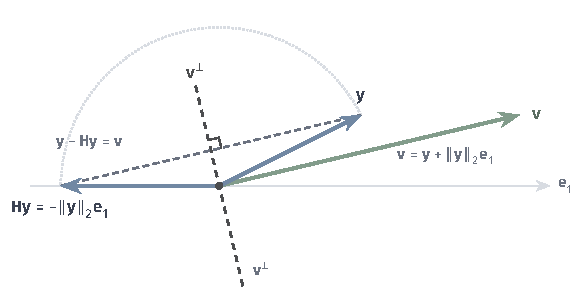
\includegraphics[width=98.94mm]{figures/01-basic-mathematics/03-vectors-matrices-and-multivariate-functions/tikz/c5-householder-reflection/figure.pdf}
  \caption{Householder反射的几何。取$\bm y=(2,1)^\top$，按式~\eqref{eq:ls-householder}令$\bm v=\bm y+\sqrt5\,\bm e_1$。反射超平面$\bm v^\perp$是$\bm y$与$\bm H\bm y=-\sqrt5\,\bm e_1$连线的垂直平分线，两者之差恰为$\bm v$；点线圆弧表示反射保持长度。解析式构造。}
  \label{fig:ls-householder-reflection}
\end{figure}

希望$\bm H\bm y=\alpha\bm e_1$。正交变换保持长度，所以必须$\alpha^2=\bm y^\top\bm y$，即$\alpha=\pm\lVert\bm y\rVert_2$。反射把$\bm y$变成$\bm y-\bm v\cdot 2(\bm v^\top\bm y)/(\bm v^\top\bm v)$，结果要等于$\alpha\bm e_1$，自然的选择是$\bm v=\bm y-\alpha\bm e_1$。验证这一选择：
\[
 \bm v^\top\bm v=\bm y^\top\bm y-2\alpha y_1+\alpha^2=2(\bm y^\top\bm y-\alpha y_1),\qquad
 \bm v^\top\bm y=\bm y^\top\bm y-\alpha y_1,
\]
所以$2(\bm v^\top\bm y)/(\bm v^\top\bm v)=1$，$\bm H\bm y=\bm y-\bm v=\alpha\bm e_1$。

符号的选择影响数值精度。$\bm v$的首分量是$y_1-\alpha$；若$\alpha$与$y_1$同号且$\bm y$接近$\bm e_1$方向，这是两个相近数相减，会严重相消。因此取$\alpha=-s\lVert\bm y\rVert_2$，其中$y_1\geq0$时$s=1$、$y_1<0$时$s=-1$，即
\begin{equation}
 \bm v=\bm y+s\lVert\bm y\rVert_2\bm e_1,\qquad
 \bm H=\bm I-\frac{2\bm v\bm v^\top}{\bm v^\top\bm v},
 \label{eq:ls-householder}
\end{equation}
这样$v_1=y_1+s\lVert\bm y\rVert_2$是两个同号数相加。作用于其他向量时不形成稠密的$\bm H$：令$\tau=2/(\bm v^\top\bm v)$，对任意向量或矩阵$\bm Z$都有$\bm H\bm Z=\bm Z-\bm v\bigl(\tau\,\bm v^\top\bm Z\bigr)$，右端也用同一公式更新。

\paragraph{算法实现与算例}
对满列秩的$\bm A\in\mathbb R^{m\times d}$（$m\geq d$），先令工作矩阵$\bm F=\bm A$、工作右端$\bm c=\bm b$，保持原列顺序，按$k=1,\ldots,d$重复下面两步。

第一步构造反射向量。取当前列段$\bm y=\bm F_{k:m,k}$，按式~\eqref{eq:ls-householder}构造$\bm v$与$\tau$，保存这一反射记录。由下面的引理，$\bm H\bm y=-s\lVert\bm y\rVert_2\bm e_1$，该列下方的元素被消去。$\bm y=\bm0$时本步取恒等变换，并记录这一列没有提供新的方向（这意味着秩亏）；对角线下方已经全为零时，也可以取恒等变换，保持该列不变。

第二步作用于剩余子块。把同一个$\bm H$作用于剩余子块$\bm F_{k:m,k:d}$的各列和右端$\bm c_{k:m}$，每个向量都按
\[
 \bm z\mapsto\bm z-\frac{2\bm v(\bm v^\top\bm z)}{\bm v^\top\bm v}
\]
计算，只需一次内积和一次向量更新；恒等变换时直接跳过。全部列完成后，取$\bm R=\bm F_{1:d,1:d}$，检查对角元非零，再用回代求解$\bm R\hat{\bm x}=\bm c_{1:d}$，输出$\hat{\bm x}$；$\lVert\bm c_{d+1:m}\rVert_2$是最小残差范数。

\begin{example}[一步反射完成的三角化]
\label{ex:ls-householder-one-step}
取$\bm A=\left[\begin{smallmatrix}3&1\\4&3\\0&0\end{smallmatrix}\right]$，$\bm b=(4,7,2)^\top$。首列$\bm y=(3,4,0)^\top$的范数为$5$，$y_1>0$，取$s=1$，于是$\bm v=(8,4,0)^\top$，$\bm v^\top\bm v=80$，$\tau=1/40$，对应的反射矩阵为
\[
 \bm H=\bm I-\tfrac1{40}\bm v\bm v^\top=\begin{bmatrix}-\tfrac35&-\tfrac45&0\\-\tfrac45&\tfrac35&0\\0&0&1\end{bmatrix}.
\]
逐列更新：第二列$(1,3,0)^\top$与$\bm v$的内积为$20$，更新为$(1,3,0)^\top-\tfrac{20}{40}(8,4,0)^\top=(-3,1,0)^\top$；右端与$\bm v$的内积为$60$，更新为$(4,7,2)^\top-\tfrac{60}{40}(8,4,0)^\top=(-8,1,2)^\top$。于是
\[
 \bm H\bm A=\begin{bmatrix}-5&-3\\0&1\\0&0\end{bmatrix},\qquad \bm H\bm b=(-8,1,2)^\top .
\]
第二列对角线下方已经为零，第二步取恒等变换。回代得$\hat x_2=1$，$\hat x_1=(-8+3\cdot1)/(-5)=1$；变换后右端的第三个分量$2$无法拟合，它就是最小残差范数。核验时，$\bm H^\top\bm H=\bm I$，原残差$\bm r=\bm b-\bm A\hat{\bm x}=(0,0,2)^\top$满足$\bm A^\top\bm r=\bm0$。这里$\bm R$的对角元为负，不影响求解；若要统一成正对角，须把$\bm R$的相应行与变换后右端的相应分量同时变号。
\end{example}

\begin{example}[直线拟合的Householder三角化]
\label{ex:ls-householder-line-fit}
再用Householder变换处理示例~\ref{ex:ls-line-least-squares}的直线拟合，$\bm A=\left[\begin{smallmatrix}1&0\\1&1\\1&2\end{smallmatrix}\right]$、$\bm b=(1,2,2)^\top$，并与正规方程法对照。第一步$\bm y=(1,1,1)^\top$，$\lVert\bm y\rVert_2=\sqrt3$，$s=1$，$\bm v=(1+\sqrt3,1,1)^\top$，$\bm v^\top\bm v=6+2\sqrt3$。第一列变为$(-\sqrt3,0,0)^\top$；第二列$(0,1,2)^\top$与$\bm v$的内积为$3$，更新为$(-\sqrt3,\tfrac{\sqrt3-1}2,\tfrac{\sqrt3+1}2)^\top$；右端更新为$(-\tfrac5{\sqrt3},\tfrac1{\sqrt3},\tfrac1{\sqrt3})^\top$。三个向量的长度平方仍为$3$、$5$、$9$，与变换前相同，这是反射保持长度的直接检验。

第二步作用于后两行，$\bm y=(\tfrac{\sqrt3-1}2,\tfrac{\sqrt3+1}2)^\top$，$\lVert\bm y\rVert_2=\sqrt2$，反射后$r_{2,2}=-\sqrt2$，右端后两分量变为$(-\tfrac1{\sqrt2},-\tfrac1{\sqrt6})^\top$。于是
\[
 \bm R=\begin{bmatrix}-\sqrt3&-\sqrt3\\0&-\sqrt2\end{bmatrix},\qquad
 \bm c_1=\Bigl(-\frac5{\sqrt3},-\frac1{\sqrt2}\Bigr)^{\!\top},
\]
回代得$\hat x_2=1/2$，$\hat x_1=5/3-1/2=7/6$，与示例~\ref{ex:ls-line-least-squares}一致；$\lvert c_3\rvert=1/\sqrt6$正是最小残差范数。$\bm R$与示例~\ref{ex:ls-normal-equations-line-fit}的Cholesky因子$\bm L^\top$只差各行的符号。
\end{example}

\paragraph{算法分析}
单步消元的依据是下面的引理。

\begin{lemma}[Householder反射]
\label{lem:ls-householder-reflection}
设$\bm y\neq\bm0$，$\bm v$与$\bm H$由式~\eqref{eq:ls-householder}给出。则$\bm H$对称正交，且$\bm H\bm y=-s\lVert\bm y\rVert_2\bm e_1$。
\end{lemma}
\begin{proof}
$\bm H$显然对称；$\bm H^2=\bm I-4\bm v\bm v^\top/(\bm v^\top\bm v)+4\bm v(\bm v^\top\bm v)\bm v^\top/(\bm v^\top\bm v)^2=\bm I$，所以$\bm H^\top\bm H=\bm I$。由$s^2=1$与$sy_1=\lvert y_1\rvert$，
\[
 \bm v^\top\bm v=2\lVert\bm y\rVert_2^2+2\lVert\bm y\rVert_2\lvert y_1\rvert=2\bm v^\top\bm y>0,
\]
于是$\bm H\bm y=\bm y-\bm v=-s\lVert\bm y\rVert_2\bm e_1$。
\end{proof}

每个$\bm H$嵌入$m$阶后只作用于第$k$至$m$行；前$k-1$列在这些行上已经是零，反射后仍为零。所以旧的零结构保持不变，$d$步后$\bm F=\bm H_d\cdots\bm H_1\bm A$是上三角矩阵，$\bm c=\bm H_d\cdots\bm H_1\bm b$。这正是取$\bm Q^\top=\bm H_d\cdots\bm H_1$的QR分解，由定理~\ref{thm:ls-qr-least-squares}，回代所得即最小二乘解。

符号$s$取与$y_1$相同，使$\bm v$的首分量是两个同号数相加，避免了主要思想中指出的相消。Householder QR后向稳定（第~\ref{sec:ls-numerical-stability}节），算出的$\bm Q$在舍入误差范围内保持正交，主要工作约为$2md^2-\tfrac23d^3$次运算。列主元可以辅助辨认近相关的列，但秩亏时的最小范数选择仍回到第~\ref{sec:ls-svd-solve}节。

\subsection{Givens旋转}
\label{sec:ls-givens}

\paragraph{主要思想}
Householder反射一次消去一整列的下方元素。若矩阵在对角线以下只有少数非零元，更经济的做法是每次只消去一个指定元素。\term{Givens旋转}（Givens rotation）在两个坐标构成的平面内旋转，其余坐标不变；每次只混合两行，消去其中一个元素。图~\ref{fig:ls-givens-householder-elimination}把旋转与反射并置。

\begin{figure*}[htbp]
  \centering
  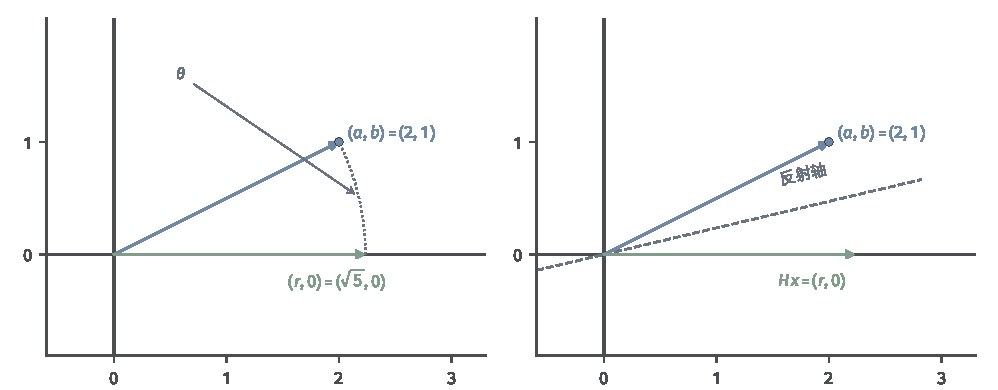
\includegraphics[width=168.998mm]{figures/00-shared/mathematical-preliminaries-upper/02-linear-spaces/matplotlib/ls-givens-householder-elimination/ls-givens-householder-elimination.pdf}
  \caption{两种初等正交消元。左：Givens旋转把$(a,b)=(2,1)^\top$沿圆弧旋到
  $(r,0)^\top$，$r=\sqrt5$，旋转角$\theta=\arctan(1/2)$；右：Householder反射沿角平分线
  把同一向量映到$(r,0)^\top$。两者都是正交变换，保持长度，区别在旋转（行列式$+1$）与
  反射（对称正交）。图中的反射取与式~\eqref{eq:ls-householder}相反的符号，精确算术中两种选择都可以。解析式教学构造。}
  \label{fig:ls-givens-householder-elimination}
\end{figure*}

先看二维问题：给定$(\alpha,\beta)^\top\neq\bm0$，求旋转$\bm G=\left[\begin{smallmatrix}c&s\\-s&c\end{smallmatrix}\right]$，$c^2+s^2=1$，使$\bm G(\alpha,\beta)^\top=(\rho,0)^\top$。第二个分量为零要求$-s\alpha+c\beta=0$，即$(c,s)$与$(\alpha,\beta)$平行；再由$c^2+s^2=1$并取$\rho>0$，得
\begin{equation}
 \begin{gathered}
 \rho=\sqrt{\alpha^2+\beta^2},\qquad c=\alpha/\rho,\qquad s=\beta/\rho,\\
 \bm G=\begin{bmatrix}c&s\\-s&c\end{bmatrix}.
 \end{gathered}
 \label{eq:ls-givens}
\end{equation}
长度不变给出$\rho=\sqrt{\alpha^2+\beta^2}$，也可以直接验证$c\alpha+s\beta=(\alpha^2+\beta^2)/\rho=\rho$。这里的$s$与Householder反射中的符号无关。$\alpha=\beta=0$时取恒等变换。

对矩阵的两行$p,q$同时作用时，新的两行是
\[
 \text{第}p\text{行}\leftarrow c\cdot(\text{第}p\text{行})+s\cdot(\text{第}q\text{行}),\qquad
 \text{第}q\text{行}\leftarrow -s\cdot(\text{第}p\text{行})+c\cdot(\text{第}q\text{行}).
\]
两式必须读取同一对旧行；若先覆盖第$p$行再用它计算第$q$行，结果就不再是旋转。右端的两个分量也按同样的方式更新。

\paragraph{算法实现与算例}
输入满列秩的$\bm A\in\mathbb R^{m\times d}$（$m\geq d$）和$\bm b\in\mathbb R^m$。先令$\bm F=\bm A$、$\bm t=\bm b$，右端记作$\bm t$是为了不与旋转参数$c$混淆。按$k=1,\ldots,d$处理各列；在第$k$列中按$i=m,m-1,\ldots,k+1$自下而上消去$f_{i,k}$，每次使用相邻的第$i-1$、$i$两行。

每次消元先构造旋转：若$f_{i,k}=0$，直接跳过；否则令$\alpha=f_{i-1,k}$、$\beta=f_{i,k}$，按式~\eqref{eq:ls-givens}计算$\rho,c,s$。为避免上溢或下溢，平方和可以先除以$\max(\lvert\alpha\rvert,\lvert\beta\rvert)$，开方后再恢复尺度，许多程序库以hypot函数提供这一计算；两分量同时为零的情形已在跳过时排除，不会出现除以零。

然后用同一个$\bm G$左乘$\bm F$的第$i-1$、$i$两行在第$k$列及以后的部分，并同步变换$(t_{i-1},t_i)^\top$，计算时先用临时量保存两行的旧值。第$k$列的这两个元素由此变成$(\rho,0)^\top$。接着继续向上消元，第$k$列完成后再进入下一列；保存旋转的顺序，就保存了$\bm Q$。全部列完成后，取$\bm R=\bm F_{1:d,1:d}$，用回代求解$\bm R\hat{\bm x}=\bm t_{1:d}$，输出$\hat{\bm x}$，并用原始数据检查残差。

新增观测时的更新最能体现局部消元的好处。设已经有$d$阶上三角的$\bm R$和$\bm c_1$，新到一条观测行$\bm w^\top$及其右端$\eta$。把新行排在$\bm R$下方，依次用$\bm R$的第$1,\ldots,d$行与它作旋转：第$k$次旋转消去新行的第$k$个元素，同时旋转$\bm c_1$的第$k$个分量与新右端。$d$次旋转后新行全为零，得到更新后的$\bm R$与$\bm c_1$，再回代即得新的$\hat{\bm x}$。这一过程约需$3d^2$次运算，也不需要旧的观测行；重新处理全部$m+1$条观测则需$O(md^2)$。

\begin{example}[一次旋转完成的三角化]
\label{ex:ls-givens-one-step}
沿用示例~\ref{ex:ls-householder-one-step}的$\bm A=\left[\begin{smallmatrix}3&1\\4&3\\0&0\end{smallmatrix}\right]$与$\bm b=(4,7,2)^\top$。第一列自下而上处理：$f_{3,1}=0$，跳过；再用第$1$、$2$行消去$f_{2,1}=4$，$\alpha=3$、$\beta=4$，$\rho=5$，$c=\tfrac35$，$s=\tfrac45$。第二列的两个元素更新为$\tfrac35\cdot1+\tfrac45\cdot3=3$与$-\tfrac45\cdot1+\tfrac35\cdot3=1$；右端更新为$\tfrac35\cdot4+\tfrac45\cdot7=8$与$-\tfrac45\cdot4+\tfrac35\cdot7=1$。第二列的$f_{3,2}=0$，跳过。

于是变换后的矩阵为$\left[\begin{smallmatrix}5&3\\0&1\\0&0\end{smallmatrix}\right]$，右端为$(8,1,2)^\top$，回代得$\hat{\bm x}=(1,1)^\top$，原残差仍为$(0,0,2)^\top$。与示例~\ref{ex:ls-householder-one-step}对照，正交因子和$\bm R$的对角符号不同，但解与最小残差相同。
\end{example}

\begin{example}[直线拟合的Givens三角化]
\label{ex:ls-givens-line-fit}
仍取$\bm A=\left[\begin{smallmatrix}1&0\\1&1\\1&2\end{smallmatrix}\right]$、$\bm b=(1,2,2)^\top$，把右端写在增广列中。第一列先用第$2$、$3$行消去$f_{3,1}$：$\alpha=\beta=1$，$\rho=\sqrt2$，$c=s=1/\sqrt2$，两行变为$(\sqrt2,\tfrac3{\sqrt2}\mid2\sqrt2)$与$(0,\tfrac1{\sqrt2}\mid0)$。再用第$1$、$2$行消去$f_{2,1}=\sqrt2$：$\rho=\sqrt3$，$c=1/\sqrt3$，$s=\sqrt{2/3}$，两行变为$(\sqrt3,\sqrt3\mid\tfrac5{\sqrt3})$与$(0,\sqrt{3/2}\mid\sqrt{2/3})$。

第二列用第$2$、$3$行消去$f_{3,2}=1/\sqrt2$：$\rho=\sqrt2$，$c=\sqrt3/2$，$s=1/2$，两行变为$(0,\sqrt2\mid\tfrac1{\sqrt2})$与$(0,0\mid-\tfrac1{\sqrt6})$。于是$\bm R=\left[\begin{smallmatrix}\sqrt3&\sqrt3\\0&\sqrt2\end{smallmatrix}\right]$，$\bm t_{1:2}=(5/\sqrt3,1/\sqrt2)^\top$，回代得$\hat{\bm x}=(7/6,1/2)^\top$。三次旋转后$\bm R$恰为Cholesky因子$\bm L^\top$，$\lvert t_3\rvert=1/\sqrt6$为最小残差范数。
\end{example}

\paragraph{算法分析}
每次旋转满足$c^2+s^2=1$，所以$\bm G$正交，并且$c\alpha+s\beta=\rho$、$-s\alpha+c\beta=0$。处理第$k$列时，参与旋转的两行在前$k-1$列上已经是零，旋转后仍为零；在第$k$列内，第$i$行被消零以后，后续旋转只涉及更上面的行对，不再改动它。因此新零不会被后续旋转破坏，结束时$\bm F$是上三角矩阵，$\bm t$是对$\bm b$施加同一串旋转的结果，由定理~\ref{thm:ls-qr-least-squares}，回代所得即最小二乘解。

Givens QR同样后向稳定（第~\ref{sec:ls-numerical-stability}节）。稠密时第$k$列需要$m-k$次旋转，总工作约为$3md^2-d^3$次运算，约为Householder的$1.5$倍；带状、上Hessenberg或局部更新的问题需要的旋转少得多，代价随之降低。可见Givens与Householder的选择依据是矩阵结构与更新方式：稠密矩阵一次性分解用Householder更省，局部结构和逐行更新用Givens更合适。

\section{SVD求解}
\label{sec:ls-svd-solve}

秩亏或秩未知时，正规方程与QR回代都不再适用。本节以最小二乘解中的最小范数解为目标，依次讲清SVD求解的主要思想、算法实现和算法分析，再分别讨论加权最小二乘与齐次最小二乘。SVD的形式已在第~\ref{chap:singular-value-decomposition}章建立；数值分解调用直接作用于$\bm A$的SVD过程，本节只说明取得因子后怎样得到解，重点是由分解构造解，而不是重新证明分解存在。

\subsection{主要思想}

SVD在输入端和输出端各给出一组标准正交方向。在这两组坐标下，$\bm A$只是把第$i$个输入坐标乘以$\sigma_i$，送到第$i$个输出坐标。于是把可拟合的输出坐标除以对应的正奇异值，就得到产生它们所需的输入坐标；零空间方向的坐标不影响拟合值，令它们为零，就得到范数最小的解。图~\ref{fig:ls-svd-solve-coordinates}画出了这一坐标变换。

\begin{figure}[htbp]
  \centering
  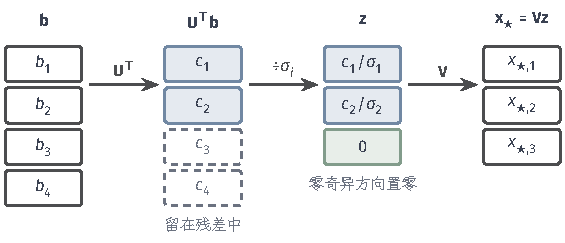
\includegraphics[width=95.652mm]{figures/01-basic-mathematics/03-vectors-matrices-and-multivariate-functions/tikz/c5-svd-solve-coordinates/figure.pdf}
  \caption{SVD求解的坐标变换，示意$m=4$、$d=3$、$r=2$。右端先变到左奇异坐标，蓝色的前$r$个坐标可以拟合，虚线框中的其余坐标无论怎样选$\bm x$都留在残差中；可拟合坐标除以对应奇异值，零奇异方向的坐标取零；最后由右奇异向量还原为原变量。}
  \label{fig:ls-svd-solve-coordinates}
\end{figure}

\paragraph{目标在奇异坐标下分离}
设$\operatorname{rank}\bm A=r$，写完整的奇异值分解$\bm A=\bm U\bm\Sigma\bm V^\top$，其中$\bm U\in\mathbb R^{m\times m}$与$\bm V\in\mathbb R^{d\times d}$正交，$\bm\Sigma$的前$r$个对角元$\sigma_1\geq\cdots\geq\sigma_r>0$，其余为零。令$\bm z=\bm V^\top\bm x$、$\bm c=\bm U^\top\bm b$。由$\bm U^\top$保持长度，
\[
 \lVert\bm b-\bm A\bm x\rVert_2^2=\lVert\bm c-\bm\Sigma\bm z\rVert_2^2
 =\sum_{i=1}^r(c_i-\sigma_iz_i)^2+\sum_{i=r+1}^mc_i^2 .
\]
输入坐标$z_{r+1},\ldots,z_d$根本不出现在目标中。

\paragraph{逐个坐标求解}
各平方项互不耦合，可以分别取最小。对每个正奇异值令$c_i-\sigma_iz_i=0$，得$z_i=c_i/\sigma_i$；输出端$i>r$的分量$c_i$无论怎样选$\bm x$都留在残差中。所以最小二乘解的全部自由度恰好是输入零空间方向上的坐标$z_{r+1},\ldots,z_d$。

\paragraph{取最小范数}
再由$\lVert\bm x\rVert_2=\lVert\bm V\bm z\rVert_2=\lVert\bm z\rVert_2$，令全部自由坐标为零就使范数最小，得到
\[
 \bm x_\star=\sum_{i=1}^r\frac{\bm u_i^\top\bm b}{\sigma_i}\bm v_i .
\]
这给出了执行顺序：先把右端投影到输出奇异方向，再对正奇异值取逆，最后由输入奇异方向重建。

\subsection{算法实现}

输入$\bm A\in\mathbb R^{m\times d}$与$\bm b\in\mathbb R^m$，不要求满秩，输出最小范数最小二乘解$\bm x_\star$，没有额外需要选定的规则。这里按精确的秩$r$描述求解；有限精度下怎样判定数值秩，以及是否截断小奇异值，属于第~\ref{chap:solution-error-regularization}章的内容（第~\ref{sec:ls-pseudoinverse-rank-change}节与第~\ref{sec:ls-tsvd-solve}节）。

\paragraph{计算SVD}
第一步调用数值SVD过程，按第~\ref{chap:singular-value-decomposition}章的形式取得$\bm A=\bm U_r\bm\Sigma_r\bm V_r^\top$。其中$r=\operatorname{rank}\bm A$，$\bm U_r=[\bm u_1,\ldots,\bm u_r]$与$\bm V_r=[\bm v_1,\ldots,\bm v_r]$的列标准正交，$\bm\Sigma_r=\operatorname{diag}(\sigma_1,\ldots,\sigma_r)$且各$\sigma_i>0$。若$\bm A=\bm0$，则直接取$\bm x_\star=\bm0$并结束。

\paragraph{投影右端}
然后计算$\bm c=\bm U_r^\top\bm b$，即$c_i=\bm u_i^\top\bm b$，$i=1,\ldots,r$。这一步把右端投影到能够拟合的输出方向上；$\bm b$在其余方向上的部分，无论怎样选$\bm x$都会留在残差中。

\paragraph{按奇异值缩放}
接着对每个$i=1,\ldots,r$计算$z_i=c_i/\sigma_i$，得到产生这些输出所需的输入坐标。除法只对正奇异值进行，零奇异值对应的方向不参与。

\paragraph{还原原变量}
最后计算
\[
 \bm x_\star=\bm V_r\bm z=\sum_{i=1}^r\frac{\bm u_i^\top\bm b}{\sigma_i}\bm v_i
\]
并输出，把奇异坐标还原为原变量。整个过程只用到因子对向量的作用，无需形成完整的伪逆。

\begin{example}[秩一矩阵的SVD求解]
\label{ex:ls-svd-solve-rank-one}
取$\bm A=\left[\begin{smallmatrix}1&1\\1&1\end{smallmatrix}\right]$、$\bm b=(1,3)^\top$。两个方程要求$x_1+x_2$同时等于$1$和$3$，方程不相容；$\bm A$的秩为$1$，解也不唯一。唯一的正奇异值为$\sigma_1=2$，$\bm u_1=\bm v_1=(1,1)^\top/\sqrt2$。按投影、缩放、还原三步，得$c_1=\bm u_1^\top\bm b=2\sqrt2$，$z_1=c_1/\sigma_1=\sqrt2$，$\bm x_\star=z_1\bm v_1=(1,1)^\top$。

两次选择都可以核对。拟合值$\bm A\bm x_\star=(2,2)^\top$取两个观测的平均，残差$(-1,1)^\top$与列空间方向$(1,1)^\top$正交，长度$\sqrt2$等于$\bm b$在被舍弃方向$\bm u_2=(1,-1)^\top/\sqrt2$上的分量的绝对值。另一方面，$\bm x_\star$与核方向$(1,-1)^\top$正交：全部最小二乘解为$(1+t,1-t)^\top$，其中$t=0$时范数最小。
\end{example}

上例是方阵，输出端被舍弃的只有一个方向。下例的矩阵更高，输出端有两个方向无法拟合，用来分别观察两类被舍弃的分量。

\begin{example}[秩亏且不相容的高矩阵]
\label{ex:ls-svd-solve-tall}
取$\bm A=\left[\begin{smallmatrix}1&1\\0&0\\0&0\end{smallmatrix}\right]$、$\bm b=(2,1,0)^\top$。唯一的正奇异值为$\sigma_1=\sqrt2$，对应$\bm u_1=(1,0,0)^\top$、$\bm v_1=(1,1)^\top/\sqrt2$。投影得$c_1=2$，缩放得$z_1=2/\sqrt2=\sqrt2$，重建得$\bm x_\star=\sqrt2\,\bm v_1=(1,1)^\top$。

输出端的第二、三个坐标属于不可拟合部分，其中第二个坐标留下残差$\bm r=\bm b-\bm A\bm x_\star=(0,1,0)^\top$。输入端的零空间为$\operatorname{span}\{(1,-1)^\top\}$，全部最小二乘解为$(1+t,1-t)^\top$，范数平方为$2+2t^2$，所选的$t=0$确为最小。用原矩阵核验：$\bm A^\top\bm r=\bm0$说明是最小二乘解，$\bm x_\star\perp(1,-1)^\top$说明是最小范数代表。
\end{example}

\subsection{算法分析}

\paragraph{正确性}
上述四步算出的正是伪逆作用于右端的结果。

\begin{theorem}[SVD求解给出\texorpdfstring{$\bm A^\dagger\bm b$}{A+b}]
\label{thm:ls-svd-solve}
对任意$\bm A\in\mathbb R^{m\times d}$与$\bm b\in\mathbb R^m$，上述过程的输出$\bm x_\star=\bm A^\dagger\bm b$，它是唯一的最小范数最小二乘解。
\end{theorem}
\begin{proof}
由式~\eqref{eq:matrix-analysis-pseudoinverse}，$\bm A^\dagger\bm b=\sum_{i\leq r}\bm v_i\bm u_i^\top\bm b/\sigma_i$，与输出相同；$\bm A=\bm0$时两者都是$\bm0$。最优性由定理~\ref{thm:matrix-analysis-pseudoinverse-minimum-norm}给出。也可以直接验证：残差$\bm b-\bm A\bm x_\star=\bm b-\bm U_r\bm U_r^\top\bm b$与列空间正交，所以$\bm x_\star$满足正规方程；$\bm x_\star\in\operatorname{range}(\bm V_r)=(\ker\bm A)^\perp$，由定理~\ref{thm:ls-minimum-norm-representative}，它在全部最小二乘解中范数最小。
\end{proof}

\paragraph{数值敏感度}
敏感性来自除以小奇异值。固定$\bm A$且$r>0$时，右端扰动$\delta\bm b$使解改变$\sum_{i=1}^r(\bm u_i^\top\delta\bm b)\bm v_i/\sigma_i$，其长度至多为$\lVert\delta\bm b\rVert_2/\sigma_r$，即放大倍数至多为$1/\sigma_r$。稳定地算出SVD并不能消除问题本身的病态：分解残差很小，恢复出的系数仍可能被观测误差严重放大。若为了压低放大而截去真实的正奇异值，求的就已不是$\bm A^\dagger\bm b$，这属于第~\ref{chap:solution-error-regularization}章的截断SVD与正则化。

\subsection{加权最小二乘}
\label{sec:ls-weighted-svd-solve}

\paragraph{主要思想}
第~\ref{sec:ls-weighted-ls}节的加权最小二乘以对称正定的权矩阵$\bm M\in\mathbb R^{m\times m}$规定目标函数$(\bm A\bm x-\bm b)^\top\bm M(\bm A\bm x-\bm b)$。核心做法是把权矩阵写成$\bm M=\bm R^\top\bm R$，于是目标函数等于$\lVert\bm R\bm A\bm x-\bm R\bm b\rVert_2^2$，用同一个$\bm R$变换$\bm A$和$\bm b$后，就成为普通最小二乘。若Cholesky分解写作$\bm M=\bm L\bm L^\top$，这里必须取$\bm R=\bm L^\top$，才有$\bm R^\top\bm R=\bm L\bm L^\top$；取$\bm R=\bm L$则得到$\bm L^\top\bm L$，一般不等于$\bm M$。

变换只作用于观测端，未知量$\bm x$本身没有改变。因此对$\widetilde{\bm A}=\bm R\bm A$、$\widetilde{\bm b}=\bm R\bm b$调用SVD求解，得到的$\widetilde{\bm A}^\dagger\widetilde{\bm b}$是加权最小二乘解中欧氏范数最小的代表。权矩阵度量的是残差，不是系数，所以不能再把它当成系数范数的权重。

\paragraph{算法实现与算例}
输入$\bm A$、$\bm b$与权矩阵$\bm M$，输出加权最小二乘解中欧氏范数最小的代表$\bm x_\star$。第一步构造权因子：用第~\ref{sec:ls-cholesky}节的方法作Cholesky分解$\bm M=\bm L\bm L^\top$，取$\bm R=\bm L^\top$；对角权$\bm M=\operatorname{diag}(w_1,\ldots,w_m)$则直接取$\bm R=\operatorname{diag}(\sqrt{w_1},\ldots,\sqrt{w_m})$。若权以$\bm M=\bm\Gamma^{-1}$的形式给出，$\bm\Gamma$为对称正定矩阵（例如观测误差的协方差），就改为分解$\bm\Gamma=\bm L\bm L^\top$，这时$\bm M=\bm L^{-\top}\bm L^{-1}$，取$\bm R=\bm L^{-1}$。

第二步白化数据，计算$\widetilde{\bm A}=\bm R\bm A$和$\widetilde{\bm b}=\bm R\bm b$。在$\bm M=\bm\Gamma^{-1}$的形式下，对$\bm A$的各列和$\bm b$用前代求解$\bm L\widetilde{\bm A}=\bm A$与$\bm L\widetilde{\bm b}=\bm b$，不显式求逆。

第三步对$(\widetilde{\bm A},\widetilde{\bm b})$调用上面的SVD求解过程，得到$\bm x_\star$并输出；$\widetilde{\bm A}$满列秩时也可以调用第~\ref{sec:ls-qr-method}节的QR求解。未知量的坐标没有改变，无须另做恢复。最后用原始数据检查加权正规残差$\bm A^\top\bm M(\bm b-\bm A\bm x_\star)=\bm0$，需要最小范数时再检查$\bm x_\star\perp\ker\bm A$。

\begin{example}[两种权重下的白化求解]
\label{ex:ls-weighted-whitening-solve}
沿用示例~\ref{ex:linear-algebra-weighted-projection}的$\bm A=(1,1)^\top$、$\bm b=(2,1)^\top$、$\bm M=\operatorname{diag}(1,4)$。对角权不必作Cholesky分解，直接取$\bm R=\operatorname{diag}(1,2)$，白化得$\widetilde{\bm A}=(1,2)^\top$、$\widetilde{\bm b}=(2,2)^\top$。$\widetilde{\bm A}$只有一列，QR因子为$\bm q=(1,2)^\top/\sqrt5$、$r=\sqrt5$，于是$c_1=\bm q^\top\widetilde{\bm b}=6/\sqrt5$，回代得$x_\star=c_1/r=6/5$，与该示例中加权正规方程$5a=6$的解一致。

若取等权$\bm M=\bm I$，则$\bm R=\bm I$，同样的步骤由$\bm q=(1,1)^\top/\sqrt2$、$r=\sqrt2$、$c_1=3/\sqrt2$给出欧氏解$3/2$。两种权重只改变送入求解器的数据，QR求解的步骤完全相同。
\end{example}

上例满列秩，加权解唯一。下例秩亏，用来同时观察权重怎样改变最佳拟合值，以及伪逆怎样在加权解中选出最小范数的系数。

\begin{example}[秩亏的加权最小二乘]
\label{ex:ls-weighted-svd-rank-deficient}
取$\bm A=\left[\begin{smallmatrix}1&1\\1&1\end{smallmatrix}\right]$、$\bm b=(0,2)^\top$、$\bm M=\operatorname{diag}(1,3)$。取$\bm R=\operatorname{diag}(1,\sqrt3)$，白化得$\widetilde{\bm A}=\left[\begin{smallmatrix}1&1\\\sqrt3&\sqrt3\end{smallmatrix}\right]$、$\widetilde{\bm b}=(0,2\sqrt3)^\top$。$\widetilde{\bm A}$的秩为$1$，唯一的正奇异值为$2\sqrt2$，左、右奇异向量分别为$\tilde{\bm u}_1=(1,\sqrt3)^\top/2$与$\tilde{\bm v}_1=(1,1)^\top/\sqrt2$。

投影系数为$\tilde{\bm u}_1^\top\widetilde{\bm b}=3$，除以$2\sqrt2$再重建，得$\bm x_\star=\tfrac{3}{2\sqrt2}\cdot\tfrac1{\sqrt2}(1,1)^\top=(\tfrac34,\tfrac34)^\top$。拟合值为$(\tfrac32,\tfrac32)^\top$：两个观测的拟合值相同，取的是$0$与$2$按权重$1:3$的加权平均，而不是普通平均$1$。原残差为$\bm r=(-\tfrac32,\tfrac12)^\top$，$\bm M\bm r=(-\tfrac32,\tfrac32)^\top$，所以$\bm A^\top\bm M\bm r=\bm0$，加权残差平方为$\tfrac94+3\cdot\tfrac14=3$。系数差的方向$(1,-1)^\top$张成$\ker\bm A$，$\bm x_\star$在这个方向上的分量为零。
\end{example}

\paragraph{算法分析}
由第~\ref{sec:ls-weighted-ls}节，变换前后的目标函数逐点相等，即$(\bm A\bm x-\bm b)^\top\bm M(\bm A\bm x-\bm b)=\lVert\widetilde{\bm A}\bm x-\widetilde{\bm b}\rVert_2^2$；未知量及其欧氏范数也没有变，所以两个问题的最优解集与最小范数代表都相同（定理~\ref{thm:ls-weighted-least-squares}）。又$\bm R$可逆，$\ker\widetilde{\bm A}=\ker\bm A$，所以$\bm x_\star\perp\ker\bm A$。数值敏感度取决于$\widetilde{\bm A}=\bm R\bm A$而不是$\bm A$：权重可能改善条件，也可能使它变差，应在变换后的系统上判断。

\subsection{齐次最小二乘}
\label{sec:ls-homogeneous-svd-solve}

\paragraph{主要思想}
第~\ref{sec:linear-algebra-homogeneous-estimation}节的齐次最小二乘在$\lVert\bm x\rVert_2=1$的约束下最小化$\lVert\bm A\bm x\rVert_2$。它是$\bm b=\bm0$的情形，单位长度约束属于求解目标，用来排除无意义的零解。核心做法是选择被$\bm A$伸缩得最小的方向。

用完整的右奇异基$\bm V=[\bm v_1,\ldots,\bm v_d]$写$\bm x=\bm V\bm z$。记$\hat\sigma_i=\lVert\bm A\bm v_i\rVert_2$为第$i$个方向的伸缩量：$i\leq\min(m,d)$时它是第$i$个奇异值（可以为零），$m<d$时多出的$d-m$个方向属于零空间，伸缩量为零。因为各$\bm A\bm v_i$两两正交，
\[
 \lVert\bm x\rVert_2^2=\sum_{i=1}^dz_i^2=1,\qquad
 \lVert\bm A\bm x\rVert_2^2=\sum_{i=1}^d\hat\sigma_i^2z_i^2 .
\]
目标是平方伸缩量$\hat\sigma_i^2$以$z_i^2$为权的加权平均，所以最小值等于其中最小的一个，并且当且仅当$\bm z$只落在取得最小伸缩量的那些坐标上时达到。最小伸缩量是单重的时，实数域中的最优方向仍有$\pm\bm v_d$两个；重数大于一或零空间多于一维时，应报告整个最优子空间，而不是声称有唯一的向量。

\paragraph{算法实现与算例}
输入$\bm A\in\mathbb R^{m\times d}$，没有额外需要选定的规则，输出使$\lVert\bm A\bm x\rVert_2$最小的单位向量$\hat{\bm x}$。第一步调用数值SVD过程，取得第~\ref{chap:singular-value-decomposition}章中的完整右因子$\bm V$，各列按伸缩量从大到小排列，并检查输入维数与秩。$m<d$时奇异值只有$m$个，完整右基中多出的方向属于零空间，也要保留；薄SVD可能没有列出全部右零空间，必须补齐相应的基，不能机械地取薄SVD的最后一列。这些方向直接从$\bm A$的SVD取得，不通过显式形成$\bm A^\top\bm A$再求特征向量。

第二步取$\hat{\bm x}=\bm v_d$并输出：存在零空间时它是零空间中的单位向量，否则是最小正奇异值的右奇异向量。它已经是单位向量，无须再归一化。最小伸缩量重复时，$\bm v_d$只是最优子空间中的一个选择；$\hat{\bm x}$与$-\hat{\bm x}$表示同一组参数比例。

\begin{example}[齐次最小二乘的两种情形]
\label{ex:ls-homogeneous-svd-run}
先取$\bm A=\left[\begin{smallmatrix}3&0\\0&1\\0&0\end{smallmatrix}\right]$。目标为$\lVert\bm A\bm x\rVert_2^2=9x_1^2+x_2^2$，约束为$x_1^2+x_2^2=1$；目标等于$1+8x_1^2$，在$x_1=0$时最小，故$\hat{\bm x}=(0,\pm1)^\top$，最小残差范数为$1$，对应最小奇异值$1$的右奇异向量。零向量虽然给出零残差，却不满足单位长度约束。

再取$\bm A=\left[\begin{smallmatrix}1&0&0\\0&2&0\end{smallmatrix}\right]$。两个正奇异值为$2$和$1$，薄SVD只列出$\bm e_2$与$\bm e_1$两个右奇异向量；补齐完整右基后还有$\bm e_3$，它满足$\bm A\bm e_3=\bm0$，最小残差为零。若只看两个正奇异值而取$\bm e_1$，得到的残差范数为$1$，漏掉了真正的最小方向。
\end{example}

\paragraph{算法分析}
正确性直接来自定理~\ref{thm:ls-homogeneous-minimizers}：$\lVert\bm A\bm x\rVert_2^2=\bm x^\top\bm A^\top\bm A\bm x$在单位球面上的最小值是$\bm A^\top\bm A$的最小特征值，由对应的特征向量达到，而$\bm v_d$正是这样的向量；主要思想中的加权平均论证给出了同一结论。最优方向的敏感度由最小特征值与其余谱之间的间隙控制，可用第~\ref{sec:ls-subspace-sensitivity}节的子空间扰动界估计；最小特征值重复时，不能保证单个方向唯一。单位长度与最优性的检验按第~\ref{sec:ls-least-squares-verification}节进行。
